\documentclass[conference]{IEEEtran}
\IEEEoverridecommandlockouts
% The preceding line is only needed to identify funding in the first footnote. If that is unneeded, please comment it out.
% \usepackage{cite}
\pagenumbering{arabic}
\usepackage{xcolor}
\usepackage{listings}
\usepackage{amsmath,amssymb,amsfonts}
\usepackage{comment}
\usepackage{algorithmic}
\usepackage{tabularx}
\usepackage{multirow}
\usepackage{graphicx}
\graphicspath{ {./images/} }
\usepackage{textcomp}
\usepackage{xcolor}
\usepackage{hyperref}

\def\BibTeX{{\rm B\kern-.05em{\sc i\kern-.025em b}\kern-.08em
    T\kern-.1667em\lower.7ex\hbox{E}\kern-.125emX}}

% \def\BibTeX{{\rm B\kern-.05em{\sc i\kern-.025em b}\kern-.08em
%     T\kern-.1667em\lower.7ex\hbox{E}\kern-.125emX}}
% \usepackage[
% backend=biber,
% style=ieee,
% sorting=ynt
% ]{biblatex}
% \addbibresource{export.bib}

\begin{document}

\title{An Embedded Machine Learning Approach to Assist Navigation for People with Visual Impairments\\}

\author{
\IEEEauthorblockN{Seán Ó Fithcheallaigh (B00830189)}
\IEEEauthorblockA{\textit{Department of Computing} \\
\textit{Ulster University}\\
Belfast, N. Ireland \\
o\_fithcheallaigh-s@ulster.ac.uk}
}

\maketitle
% Next two lines will put page numbers in
\thispagestyle{plain}
\pagestyle{plain}

\begin{abstract}
TBD
\end{abstract}

\begin{IEEEkeywords}
Machine Learning, Deep Learning, Embedded Systems, The Edge, Neural Networks, Arduino
\end{IEEEkeywords}

\section{Introduction}
% This research is related to the testing and development of an obstacle avoidance and navigation system for people with sight difficulties. The initial part of this section will give background information on why systems like this are needed, and will then move into a more detailed exploration of the research.
\subsection{The lives of people dealing with sight loss}
There are over two million people in the UK who live with sight loss; where sight loss includes: people who are registered blind or partially sighted; people whose vision is better than the levels that qualify for registration; people who are awaiting or having treatment such as injections, laser treatment or surgery that may improve their sight; Correctly prescribed glasses or contact lenses could improve the sight of people who have sight loss \cite{b1}. Experts also predict that the number of people suffering from sight loss will double to over four million by 2050 \cite{b2}. The main reason for sight loss includes age-related macular degeneration (AMD), uncorrected refractive errors and cataracts \cite{b1}. 

%Of the two million people with sight loss, the leading causes of sight loss include (with the approximate number of people affected) \cite{b1}:
%\begin{itemize}
    %\item Age-related macular degeneration (AMD) (488,000 people)
    %\item Cataract (394,000 people)
    %\item Diabetic retinopathy (97,000 people)
    %\item Glaucoma (151,000 people)
    %\item Uncorrected refractive error (809,000 people)
    %\item Other eye problems (150,000 people)
%\end{itemize}

The impact of sight loss on individuals can differ based on their personal situations. Nevertheless, in the UK, many people acknowledge that individuals with visual impairments are not treated equally to those without. \cite{b1}.

% How sight loss impacts those effects can vary, depending on personal circumstances. Some factors which can be influential in a person's experience with sight loss can be: they receive support and receive it at the right time, a person's age, the presence of other disabilities, and the severity of the sight loss. However, most people in the UK agree that those with visual impairments are not treated the same as those without visual impairments, according to a key finding in \cite{b1}.

% Individuals who have visual impairments tend to avoid unfamiliar environments, which can have adverse effects on their overall health and wellness. Obstacle detection and warning can improve the mobility and safety of visually impaired people, particularly in unfamiliar environments; as one RNIB research participant said, "If there were more things in shops to help people with sight loss [...] to help us get around" \cite{b1} \cite{b2}. However, if we look around our world, we can see that transport systems are not built with the visually impaired in mind [3]. This fact is one factor likely to be a factor in four out of every ten blind people who are only able to make some of the journeys they either need to or wanted to \cite{b1}.

Individuals who have visual impairments tend to avoid unfamiliar environments, which can have adverse effects on their overall health and wellness. Obstacle detection and warning can improve the mobility and safety of visually impaired people, particularly in unfamiliar environments, which can help facilitate the journeys they need to do. However, transport systems are not built with the visually impaired in mind \cite{b2}. It is likely that this contributes to the limitation of four out of every ten blind individuals who can only complete some of the journeys they require or desire. \cite{b1}.

Visually impaired people face many issues when navigating their journey, such as understanding how to reach their destination. Typically, the route to a destination will stay the same - streets remain in the same place, and road crossings tend not to move. However, another issue they face is random obstacles placed in their path. These are things that a visually impaired person could have no way of knowing are there. Of course, aids such as the white cane can be used to assist with this kind of issue. However, not everyone may want to use a cane (potentially because of the signal that sends: I am different, I have an impairment). Another reason could be because, although a person may be registered as blind, they may still have some level of vision (as many do) and do not wish to give up a level of independence completely. 

\subsection{The Problem}
A need exists to develop systems that can assist visually impaired people in navigating their surroundings. In any proposed navigation system for the visually impaired, obstacles must first be detected and localised. Then, navigation information must be communicated to the person, allowing them to avoid obstacles. Using various modalities such as voice, tactile feedback, and vibration could facilitate the achievement of this goal.
 
This research proposes using machine learning methods within an embedded system to develop a solution that can detect obstacles in the path of a visually impaired user navigating an indoor environment. 
 
Several tasks will need to be completed to determine the system's feasibility. The first step will be the investigation of various sensor modalities in order to determine the most appropriate sensor or combination of sensors. Then a dataset will be gathered covering a range of obstacle detection and avoidance scenarios. This dataset will then be used to train, test, and validate several Deep Learning and machine learning models to understand which is best at detecting and localising obstacles. Development work will then be done to allow this model to be implemented on a constrained device, and the performance of the final model will be assessed against critical parameters.

A constrained device is something that works at "the Edge". Devices that work at the Edge will typically do any data processing and analysis on the device itself. This allows for a reduction in the time it takes for a system to get a result. This reduction in time, or latency, is critical in the system this research aims to investigate. Power is another important constraint when dealing with edge devices, and is obviously very important when developing a portable navigation system, as it will need to run under its own power. Memory is another important consideration when working at the Edge. This means that any proposed model must be able to be stored in the device's memory, and still be able to take in sensor data for processing. 

There are a lot of considerations when dealing with Edge, or constrained devices. This paper will detail the investigations and research carried out with the aim of developing a navigation system on a constrained device.

\subsection{Paper Structure}
The paper will present information on the technical aspects of machine learning at the edge, as well as presenting information on related research. From there, the discussion will move on to how the data was captured for this research and the initial analysis that was carried out using classification algorithms. From there the discussion moves on to the investigation carried out on neural networks and the deployment of the system on a constrained device. The final sections will be an evaluation and critical analysis of the research with a discussion on potential future work.

\section{Technical Review}
\subsection{Introduction}
As has been discussed, the goal is to design and build an object detection system which researchers can implement on a constrained device. This detection system will operate at what is called "the edge". In recent years, the term "edge" has been more common in discussions about the future directions of machine learning, and is often discussed in connection with the Internet of Things (IoT). When discussing machine learning at the edge, one may hear terms such as "edge AI" or "edge ML". Other standard terms would be "embedded machine learning", "embedded ML", "embedded AI", or the popular phrase: "tiny ML". All these terms are interchangeable, and while there may be some differences depending on the context, a person can use any of these terms to discuss the same topic.

% Embedded is quite a common term in the field of electronic engineering. An embedded device, or an embedded system, is a computer that controls the electronics of many of today's modern devices. We can find embedded systems in everything from mobile phones to modern cars to satellites which orbit the Earth. These embedded systems can run software that will control the system's functions and ability.
% Embedded systems are in more places than one may imagine, or it may be more accurate to say that there are more embedded chips in a single device than one may imagine. Globally, In 2020, more than 28 billion microcontrollers were shipped, and the trend is predicted to grow, with a focus on automation and artificial intelligence devices \cite{b3}. Given how common these devices are, it is pretty apparent that researching how best to transfer machine learning models to these systems is an important step.

The term 'edge' may seem slightly unusual. So how does Edge relate to machine learning? 

When discussing the internet, computers, or IT systems, most people will have an image of their PC at home or the computer they use at work. However, there are more devices connected to the internet than computers. As of 2021, research shows there were 12.2 billion active IoT connections \cite{b3}. These IoT devices cover almost any aspect of our lives that one cares to think about, everything from smartwatches; intelligent kitchen appliances; baby monitors connected to the internet, allowing parents to check in from anywhere in the world; shipping containers; and industrial sensors used to monitor the health of machinery. The list goes on and on.

How are all these billions of devices connecting to networks and communication? They are connected to servers, and these servers are often referred to as the "cloud".
These devices are connected to a network; they take readings from their sensors and send that information to a location where it can be stored and processed. From this perspective, these devices sit at the 'edge' of the network, hence the name.

\subsubsection{Edge AI}
For a long time, IoT devices have been seen as ways to collect data via onboard sensors. They would collect the data and transmit it back to a hub for processing. However, this approach is costly in several ways. First, it can cost a lot of money to transmit large amounts of data, due mainly to the connectivity and storage costs; there is also the issue that transmitting data is a highly power-hungry task for any battery-powered IoT device. Second, it is expensive in human time, too, because people will need to evaluate the data and process it, potentially making some decisions based on that data analysis.

Sending information back to a central location to be processed and then returning the result can take time, referred to as latency. The time required for this may only be a matter of seconds, which is acceptable for some applications, but would be too long for other applications where near-instant feedback is needed. An example of a time-critical system could be a system on an autonomous vehicle needing to react to traffic lights. The vehicle cannot wait a few seconds to determine if it is approaching a red light and needs to stop. 

% \subsubsection{Hardware Consideration}
% Edge AI is built on constrained devices, such as microcontrollers (MCU). Constrained devices, such as microcontrollers, are the primary platform for edge AI applications. The limited processing power, available memory and power consumption are the main factors constraining these devices. 

% The image in Fig. \ref{fig:ucblock} shows a block diagram for an edge AI device:    
% \begin{figure}[ht]
% 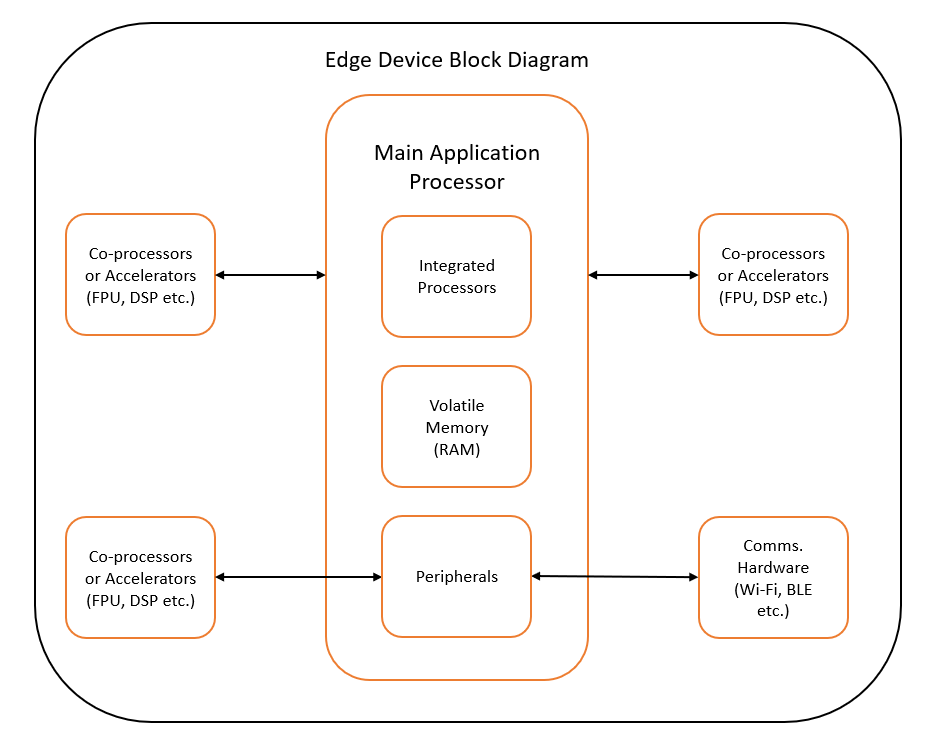
\includegraphics[width=8cm, height=6cm]{images/edge_device_block_diagram.png}
% \centering
% \caption{Block Diagram for a Constrained Device}
% \label{fig:ucblock}
% \end{figure}

% Fig \ref{fig:ucblock} shows that the processor is the centre of the whole system, with the processor being the element that runs applications and runs the algorithm for an AI application. Depending on the system, there may also be co-processors or accelerators. An accelerator is a bit of hardware designed to carry out a specific task. For example, one typical accelerator would be a floating-point unit (FPU), which will be added to a system to carry out floating-point arithmetic as quickly as possible. Other accelerators which could be common in edge AI applications would be digital signal processing (DSP) blocks and linear algebra blocks \cite{b4}. 

% There are many edge AI devices that have been designed with a specific use case, or area of use, in mind. For example, there is the Carol \cite{b5}, which is a platform developed by Google for AI applications in a production environment. The System on Module (SoM) device is a fully integrated system for accelerated machine learning applications (including CPU, GPU, Edge TPU, Wi-Fi, and Bluetooth). The Jetson Nano from NVIDIA \cite{b6}, which is an AI computer for makers, learners, and developers \cite{b7}. As discussed in \cite{b7}, the Jetson Nano allows for the use of libraries and APIs for TensorRT and cuDNN, which can be used for deep learning applications that require higher performance, CUDA for GPU accelerated applications, NVIDIA Container Runtime for containerised GPU accelerated applications, as well as APIs for sensor development or working with OpenCV. This, along with NVIDEA's other AI-focused development kits, is aimed at prototyping, before being put into production.

While a lot of high-end Edge AI devices have been developed, lower-end systems are still capable of carrying out AI applications. One example of a lower-end system is the Beaglebone AI \cite{b8}. This system is built on Linux, and based around the Texas Instruments (TI) AM5729, with a TI C66x floating point DSP, with TI embedded vision engines (EVE) \cite{b9}. Then there is the Arduino Nano 33 BLE Sense which is a small development board which is AI-enabled. The Arduino Nano 33 contains a number of onboard sensors, such as a 9-axis inertial sensor, humidity sensor, microphone and proximity sensor. The Arduino board also has GPIO pins which can allow extra sensors to be added if needed or required. The Arduino development kit allows for embedded machine learning applications to be run where models created using TensorFlow Lite can be uploaded to the board via the Arduino IDE \cite{b10}.

% Another type of hardware configuration would be the field programmable gate array (FPGA). An FPGA is an IC which allows the user to configure the hardware to meet the requirements of the project. Using FPGAs allows the developer to build a processor that is specific and tailored to running machine learning models and so on. The flexibility that FPGAs allow means they are an excellent platform for developing AI accelerators \cite{b9}. Intel has a range of FPGAs which allow real-time, low-latency, and low-power deep learning inference. A number of devices such as the Intel Cyclone. Other manufacturers are producing AI-focused FPGAs, such as Qualcomm, which has, among other systems, the Snapdragon, which is a System on Chip (SoC) which contains a CPU and GPU and is very power efficient \cite{b11}. 

\subsubsection{Software and Frameworks}
As previously discussed, when building edge AI applications on an MCU, one must give the availability of memory due consideration. Unfortunately, available memory is problematic when implementing any machine learning algorithm or neural network on an MCU because the weights and biases required for a model to function and any data points can take up large amounts of memory. Software libraries and frameworks have been developed to help reduce things like memory requirements.

The main tools or frameworks used in deep learning would be TensorFlow and its associated Keras API and PyTorch. TensorFlow, developed by Google Brain, is a powerful open-source library aimed at deep neural networks. These tools are typically optimised to run on GPUs and other specialised hardware. The reason for this is to accelerate the training processes. Once a model is trained, using that model to make inferences is less computationally expensive, which is essential for dealing with edge devices. However, it is important to note that why the inference is less computationally expensive, the MCU does not have a free ride - a reasonable amount of memory and processing power is still required to carry out the inference. To try and reduce the requirements on the front end, frameworks such as TensorFlow and PyTorch have implemented model compression techniques with little to no effect on computational accuracy \cite{b9}. 

While TensorFlow (with TensorFlow Lite) and PyTorch have been mentioned here, TensorFlow has been the main focus, because while PyTorch has PyTorch Mobile, it is aimed at mobile devices which run on either Android or iOS, whereas TensorFlow Lite can be used on embedded system \cite{b9} \cite{b12}.

TensorFlow Lite (TLF) is a set of tools that have been designed and built to allow on-board machine learning. It has been designed to help developers run models on embedded systems, as well as on mobile devices \cite{b12}.

Some of the key features of TensorFlow Lite (TFL) include:

\begin{itemize}
    \item Optimisation
    \item Multi-platform
    \item Multi-language options
    \item High performance
\end{itemize}

Process optimisation is extremely important when developing embedded machine learning systems. TFL deals with optimisation by dealing with a number of key constraints which are common to embedded systems: latency, privacy, connectivity, size, and power consumption \cite{b7}. The reduced latency comes from the fact that there is no information going to the server to be processed, and then back to the device. TFL removes a lot of privacy issues which may traditionally have been present in cloud-based machine learning tasks because no data will actually leave the device. Connectivity issues are side-stepped because the device does not need to connect to a network. Some systems may send information back to a cloud-based server, but this would become a non-critical task, in terms of timing. TFL can also reduce the size of any associated files, meaning they are more suitable for embedded applications. Power consumption is reduced through efficiencies in the interface, as well as the lack of network connection, since, typically, sending information tends to be a large drain on power.

% On the topic of multi-platform, TFL can be used to develop models that will work on Android and iOS devices, as well as on MCU and embedded Linux systems. In terms of languages, TFL has support for Python, Objective-C, C++, Java and Swift. The ability to use multiple languages is a great advantage, but the ability to optimize the models is essential to the success of TFL. This will be discussed in the following section.

\subsubsection{Optimisation} Since optimisation is key, this section will explore the topic more. Various optimisation techniques can be applied to models to allow efficient operation with the limited computational power and limited memory available on a constrained device. As previously discussed, some optimisation techniques allow for the use of accelerated inference \cite{b13}.

Models should be optimised for a number of reasons. One of the main reasons would be size reduction. There is no single method used for reducing the model size, but no matter the process, there are a number of advantages in doing this:

\begin{itemize}
    \item \textbf{Smaller storage size}: A smaller size model will take up less memory on the end device. If we take the Arduino Nano as our target device, this MCU does not come with a lot of onboard memory, so reducing the model size is critical for deployment.
    \item \textbf{Reduced memory usage}: Using a smaller model will result in less RAM being used when the model is run. This will allow other more memory to be available for other elements of the application to use. This will typically result in better performance overall.
    \item \textbf{Reduced download size}: A smaller model will need less time to download onto the end device. This is a benefit when a system might have a small window of time to receive a newly trained model.
\end{itemize}

Another reason is \textbf{latency reduction}. In the context of embedded machine learning, latency can be defined as the amount of time taken for the system to process a piece of data and make a decision based on that data. Optimisation can reduce the amount of computation needed to make this decision (or, to put it another way, reduce latency). Lower latency will also have the benefit of reducing power consumption.

Then we have \textbf{accelerators}. One consequence of model optimisation is that it can impact the model's accuracy, and this should be kept in mind during development. TFL offers tools such as Edge TPU, which can run inference extremely fast when using models which have been correctly optimised. Edge TPU is offered by Google, and is a purpose-built ASIC which has been designed specifically to run AI on edge devices, allows for high-quality machine learning inferencing at the edge and is based around the Carol development environment discussed above \cite{b14}.

As discussed, optimisation has the potential to modify the accuracy of the model, and any developer must keep this in mind during the development process. The potential inaccuracies cannot be predicted, so a method of dealing with them cannot be developed and included as part of the TFL suite of tools.

Depending on what works best for a given application, TFL offers a number of optimisation paths: quantisation, pruning, and clustering. The quantisation approach works by reducing the precision of the numbers used to represent the model parameters \cite{b13}. By default, these are set to 32-bit floating point numbers. Reducing the precision of the numbers or parameters of the model means that less memory is required, this in turn means an overall smaller model, which will result in faster computation.

From \cite{b12}, we get the quantisation techniques which are, with their benefits are:

\begin{itemize}
    \item \textbf{Post training float 16 quantisation}: This will offer a size reduction of up to 50 per cent with insignificant accuracy loss. This technique is supported on CPUs and GPUs
    \item \textbf{Post training dynamic range quantisation}: Will offer up to 75 per cent size reduction with the smallest accuracy loss. This technique will work on CPUs and GPUs (Andriod)
    \item \textbf{Post training integer quantisation}: This technique will require an unlabelled representative sample and will produce up to 75 per cent size reduction with a small accuracy loss. This technique will work on CPUs and GPUs (Android), EdgeTPU and Hexagon DSPs
    \item \textbf{Quantisation-aware training}: This technique requires labelled training data, producing a size reduction of up to 75 per cent. It offers the smallest accuract loss and can work on CPUs, GPUs (Android), EdgeTPU, Hexagon DSP
\end{itemize}


Next is pruning. Pruning is an approach which removes parameters within the model which will have only a minor impact on the prediction. A pruned model will take up the same size of memory and will have the same latency, but it can be compressed more efficiently.

Then finally there is clustering. Clustering works by grouping the weights of each layer into a predefined number of clusters, which allows for the centroid values for the weights belonging to each cluster. This means the number of unique weights is reduced, which also reduces the complexity.

\section{Literature Review}
Many articles have been written on the topic of obstacle detection, some of these, such as \cite{b15}, use mobile devices such as smartphones and tablets with in-built cameras, which run algorithms to detect the presence of obstacles. While smartphones and tablets are not the proposed constrained device used in this research, the paper offers interesting insights into the use of a small portable device which is not intrusive. The model presented in this work uses a number of sensors for detecting obstacles. The sensors listed include the onboard camera, proximity sensor, accelerometer, and gyroscope. The researchers in this work use the Canny Edge Detection algorithm \cite{b16}. This algorithm extracts useful information from vision objects and reduces the amount of data this is processed. As such, it is a common algorithm found in the area of computer vision as well as edge detection.

Other research, such as \cite{b17} offers insights into how machine learning can be used to carry out Real-Time Ranging and Localisation (RTRL) and discusses a few different approaches to labelling data which are interesting and offer a useful background to the proposed work. They use two different labelling methods – one is a simple multi-class labelling system, and the other is a grid labelling system. This work also discussed the performance of several classification models which was very informative – the authors showed that tree-based models along with Stochastic Gradient Boost performed better than linear models. The paper also discussed which of the labelling methods they investigated showed the best performance. As such, this paper contains a lot of useful information related to the proposed work.
The proposed work’s goal is to access the feasibility of a deep learning/machine learning model running on what is a constrained device. 

The work presented in \cite{b18} offers a discussion on topics like the future of Machine Learning at the edge, as well as a discussion on Machine Learning/Deep Learning algorithms, it also presents a discussion on how Machine Learning can be brought to the edge, discussing architectures and hardware, and wireless standards for Artificial Intelligence-enabled devices. As such, the work in \cite{b18} provides a wide-ranging and extremely useful background to the topic of Machine Learning and Deep Learning on constrained devices. 

The work presented in \cite{b19} used a thermal imaging camera and provides some useful insights into data collection as well as a discussion on the system architecture. The work then goes on to discuss the use of CNNs and highlighted some of the problems encountered when training on the AlexNet network – specifically lighting, which may be an issue for the work proposed here, depending on sensor type, and as such, is something to keep in mind.

Finally, a slightly older paper is presented in \cite{b20}. While this paper is older, it provides a very useful entry point into machine learning at the edge. The work discusses some of the early stages of embedded machine learning development, looking at work done using smartphones and how non-CPU processors, such as DSPs can play an important role in reducing deep networks to allow them to be used on a constrained device. The paper also discusses methods for overcoming the constraints of an embedded system, which includes a compression model which allows deep neural networks to fit and operate on embedded systems. 
Some work has been done to try and develop systems to assist people with visual impairments, however, these systems do not all use machine learning or deep learning techniques, the work is interesting as it gives some insight into the type and range of sensors used to assist visually impaired people. In \cite{b21} the author discusses using a traditional cane which some visually impaired people use and upgrading this stick by connecting it with an application which runs on a mobile phone. The authors proposed system includes the use of an ultrasonic sensor for distance measurement, a water sensor to detect rainfall or water level and a NodeMCU microcontroller. When near an obstacle or some water, the proposed system will send an alert to the user.

The authors of \cite{b22} propose a system called LineChaser, which guides the user to the end of a line while continuously reporting the distance and direction of the last person in the line, so they can be followed by the LineChaser user. The equipment used in this system is a smartphone camera, which is used to detect people nearby with the built-in infrared sensor which is used to estimate distance. As such, this work requires the user to operate and hold a smartphone while using the LineChaser system.

Other work has proposed the use of drones, such as \cite{b23} which proposes a drone-assisted navigation system to support people with visual impairments to carry out "hand-object" tasks through the use of fine-grain haptic feedback. The study shows that the drone-based approach produced greater accuracy for the user when compared to audio-based hand guidance system. 

The authors of \cite{b24} propose an object detection system for visually impaired people using machine learning. The proposed system uses computer vision and a machine learning multi-label classification approaches to recognise objects which are close to the user of the system. The system architecture uses TensorFlow and Open CV, the YOLO (Tiny and V3) algorithm and RetinaNet to detect objects in indoor and outdoor settings. Using various techniques, the authors were able to show good results in object detection.

The authors of \cite{b25} discuss a portable camera-based method to assist people with visual impairments to understand and recognise indoor objects. The authors proposed using a coarse description technique which allows the classification of multiple objects. This coarse approach has the benefit of keeping processing time low, which it does by sacrificing some information detail. The proposed system uses two techniques: Euclidean distance measurements, and semantic similarity measures which use Gaussian process estimation.

\section{System Development}
This section of the report will present information on the technical work carried out on the research project. It will start with a discussion on the data collection process, followed by a discussion on the initial analysis of that data using classification techniques from the machine learning toolbox. From there a discussion on the development of a neural network will be presented before moving on to examine the deployment of the network onto the constrained device.

\subsection{Data Collection}
A list of potential sensors was examined against a list of criteria, such as cost, accuracy, size, power consumption and so on. Each potential sensor (from LiDAR to ultrasonic sensors to cameras) was scored. This scoring showed that the best sensor, given the constraints of the research, was the ultrasonic sensor. This was teamed with the Arduino Nano 33 BLE sense development kit. The Arduino development kit offers a small, affordable system with its own IDE. The ultrasonic sensor's output can be read using the Arduino's general-purpose input/output (GPIO) pins. It was decided to use two ultrasonic sensors, to allow data collection on two channels. The image in Fig. \ref{fig:collection1} and \ref{fig:collection2} show the Arduino and the data collection system:    
\begin{figure}[ht]
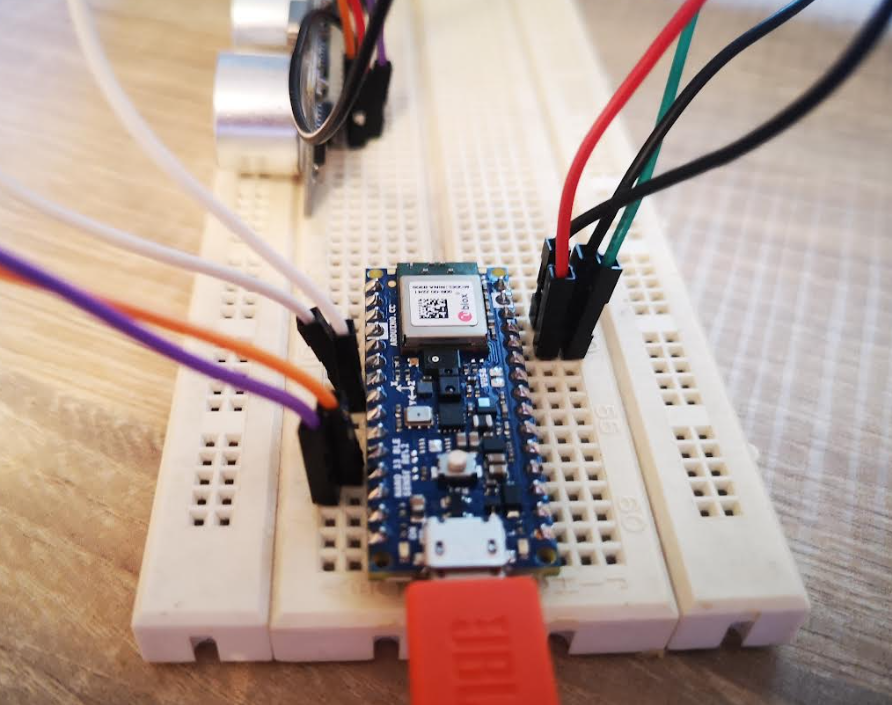
\includegraphics[width=8.5cm, height=6cm]{images/data_collection_system1.png}
\centering
\caption{Arduino Nano 33 BLE Sensor Development Kit}
\label{fig:collection1}
\end{figure}


\begin{figure}[ht]
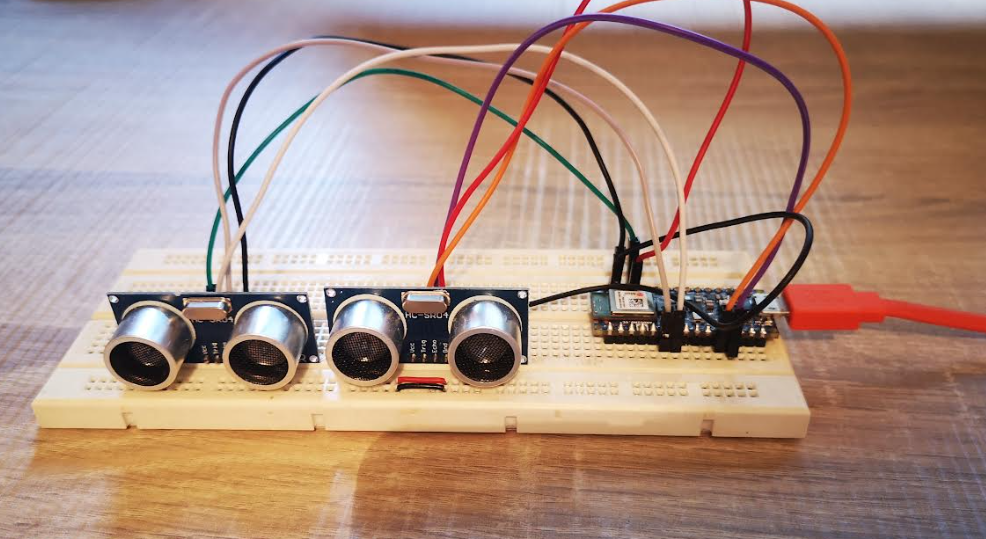
\includegraphics[width=8.5cm, height=6cm]{images/data_collection_system.png}
\centering
\caption{Arduino Nano 33 BLE Sensor Development Kit}
\label{fig:collection2}
\end{figure}

Data were collected for a number of obstacles, namely a closed door, a display stand, a storage box, and a large bin, with each obstacle placed in the centre of a hallway. These obstacles were chosen because they are reasonably large, and as such, should return strong distance measurements. 

In front of the obstacle was an imaged 3-foot by 3-foot grid. This grid was broken into 1-foot by 1-foot grids. This gives 9 grids in total, labelled 1 to 9. The data collection system will be placed in each of those 9 grids, pointing directly forward. An example of this grid is shown Fig. \ref{fig:grid1}.

\begin{figure}[ht]
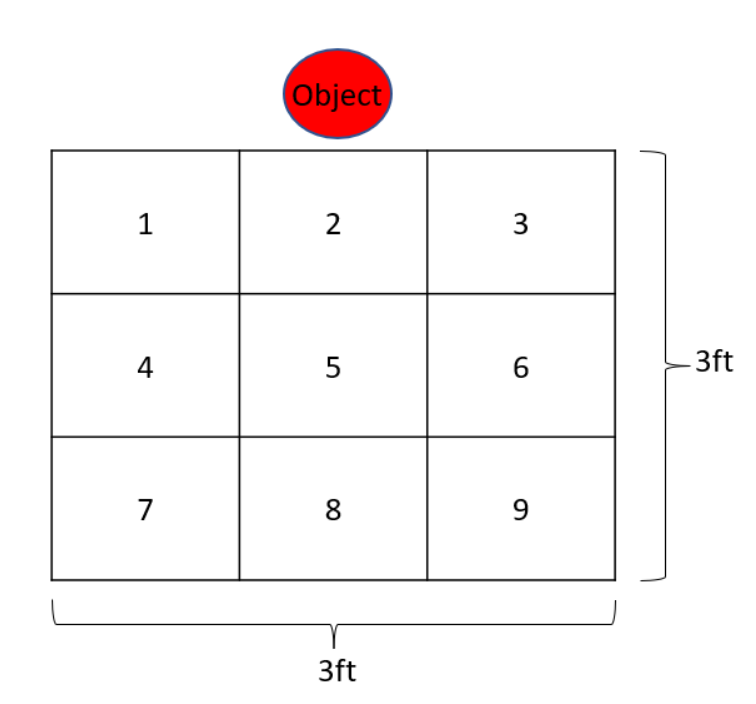
\includegraphics[width=8cm, height=7cm]{images/grid.png}
\centering
\caption{Image Depicting the Data Collection 3x3 Grid}
\label{fig:grid1}
\end{figure}




When the measurement starts, it will be sent to a serial port monitor, specifically Tera Term. Tera Term allows the user to set up a file in which the transmitted data will be saved in comma-separate values (CSV) files. As well as the obstacles, data will be collected from the hallway when there is no object in place. As well as the gathered distance measurements information was gathered on the grid location and if an object was present or not. This information was output via a program written for the Arduino. An example of the dataset headers can be seen in Table \ref{table:1}:

\begin{table}[ht]
\centering
\begin{tabular}{||c c c c||} 
 \hline
 Channel1 & Channel2 & Object & Grid \\ [0.5ex] 
 \hline\hline
 2243 & 1392 & Yes & 1 \\ 
 \hline
 2399 & 1476 & Yes & 1 \\
 \hline
 2313 & 1245 & Yes & 1 \\
 \hline
 2257 & 1388 & Yes & 1 \\ [1ex] 
 \hline
\end{tabular}
\caption{Example of Ultrasonic Dataset}
\label{table:1}
\end{table}

\subsection{Initial Analysis}
\subsubsection{Introduction}
This section of the report will give a brief overview of the initial data analysis steps taken and the results generated from this analysis. This analysis will be carried out with a focus on what is referred to as "object analysis" and "grid analysis". The purpose of object analysis is to understand how well the machine learning techniques are at determining if an object is present or not in the data. Grid analysis is trying to determine how well machine learning or deep learning techniques can be used to determine how accurate the model is at determining which grid the data was gathered from. This information would be useful for navigation (i.e. should the person move to the left or right to avoid an object).

\subsubsection{Binary Analysis}
To understand how well a system may be able to detect an object or not, an initial test was carried out on the datasets. This initial examination would be carried out by using two datasets at a time: one dataset would be a dataset for an object, and the other dataset would be data gathered for no object. 

The data was processed through a number of classification models, specifically:
\begin{itemize}
    \item Logistic Regression
    \item Decision Tree
    \item K-nearest neighbour
    \item Linear discriminant analysis
    \item Gaussian Naive Bayes
\end{itemize}

The order of the datasets tested is shown in Table \ref{table:2}:
\begin{table}[ht]
\centering
\begin{tabular}{||c c||} 
 \hline
 Dataset 1 & Dataset 2  \\ [0.5ex] 
 \hline\hline
 Display Stand & Clear Hallway  \\ 
 \hline
 Closed Door & Clear Hallway \\
 \hline
 Storage Box & Clear Hallway \\
 \hline
 Large Bin & Clear Hallway \\ [1ex] 
 \hline
\end{tabular}
\caption{Datasets test for initial analysis}
\label{table:2}
\end{table}

Using Python the two datasets were brought together into a single \texttt{DataFrame}. The data was then into training and testing datasets using \texttt{train\_test\_split} with the default settings.

The results of this analysis can be seen in Fig. \ref{fig:init_binary}
\begin{figure}[ht]
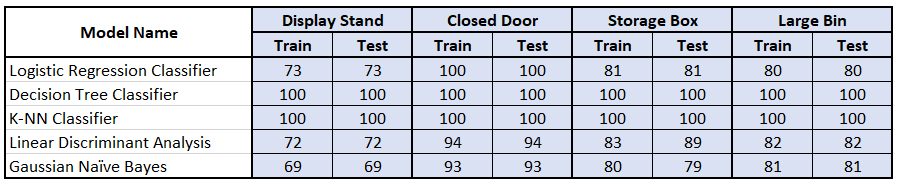
\includegraphics[width=8cm, height=3cm]{images/initial_binary_search.png}
\centering
\caption{Results, Shown as a Percentage, for the Initial Binary Search}
\label{fig:init_binary}
\end{figure}

It can be seen from the results in Fig \ref{fig:init_binary} that the \texttt{Decision Tree Classifier} and \texttt{K-NN Classifier} are producing the best accuracy scores, with 100\% accuracy, for all the test data. The lowest accuracy score was generated by the \texttt{LDA} algorithm, producing an accuracy score of 72\%. It can be seen that typically the accuracy generated for the train data and that generated for the data are the exact same. One reason for this could be that the data does not have enough variation to generate a test dataset that is sufficiently different. However, these results did provide confidence that a system could be designed to detect objects. 

\subsubsection{Grid Analysis}
The next step in the analysis process was to understand how well we can determine an object from a grid perspective. This is important as the goal is to understand if a navigation system can be deployed on a constrained device, so having the ability to understand where the object is relative to the person is key.
To complete this analysis, the datasets had to be modified. As has been discussed, there are datasets for four objects and a dataset for no object. Each dataset contained information for nine grids. The data for no object needs to be merged with the datasets for objects. This required the addition of an extra grip position, specifically grid 0. This grid 0 would represent no object. The important thing to get right here is that the datasets are balanced (i.e. the same number of samples for each grid). 

% The balanced dataset is illustrated in Table \ref{table:3}:

%\begin{table}[ht]
%\centering
%\begin{tabular}{||c c c c||} 
 %\hline
 %Channel1 & Channel2 & Object & Grid \\ [0.5ex] 
 %\hline\hline
 %7453 & 6722 & No & 0 \\ 
 %\hline
 %7528 & 6801 & No & 0 \\
 %\hline
 %7459 & 6842 & No & 0 \\
 %\hline
  %2313 & 1245 & Yes & 1 \\
 %\hline
 % 2313 & 1245 & Yes & 1 \\
 %\hline
 %2257 & 1388 & Yes & 1 \\ [1ex] 
 %\hline
%\end{tabular}
%\caption{Example of a balanced dataset}
%\label{table:3}
%\end{table}

With the balanced dataset in place, the grid analysis could be carried out. This time the response was the grid number, unlike the binary search analysis, where the presence of an object or not was the response. The data was processed through the same models listed above and the results of this analysis can be seen in Fig. \ref{fig:initial_analysis_gridsearch}.

\begin{figure}[ht]
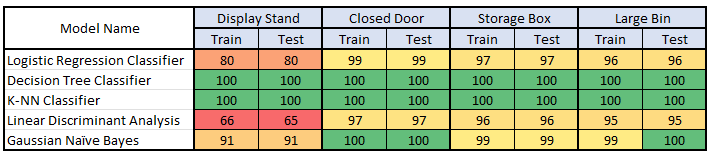
\includegraphics[width=8cm, height=3cm]{images/initial_analysis_gridsearch.png}
\centering
\caption{Results, Shown as a Percentage Value for the Grid Search}
\label{fig:initial_analysis_gridsearch}
\end{figure}

We can see from this analysis that once again, the Decision Tree Classifier and the K-Nearest Neighbour algorithms produce 100\% accuracy.  The LDA algorithm produces some of the lowest accuracy figures. However, the majority of the results are over 90 per cent. As with the binary analysis, it can be seen that the results for the train and test datasets are the same for each object. This will require further investigation.

\subsection{Using Unseen Data}
One possible explanation for the identical accuracy of the training and testing data could be that the data used for both sets are very similar. This is because the measurement system and the object being detected are static throughout the data collection process. 

To test this idea, and to look for more representative results, the algorithms will be trained on datasets from three objects, and tested on data from one object, which it has not "seen". This analysis was done for both the binary analysis and the grid analysis. The results can be seen in Fig \ref{fig:new_data_results},

\begin{figure}[ht]
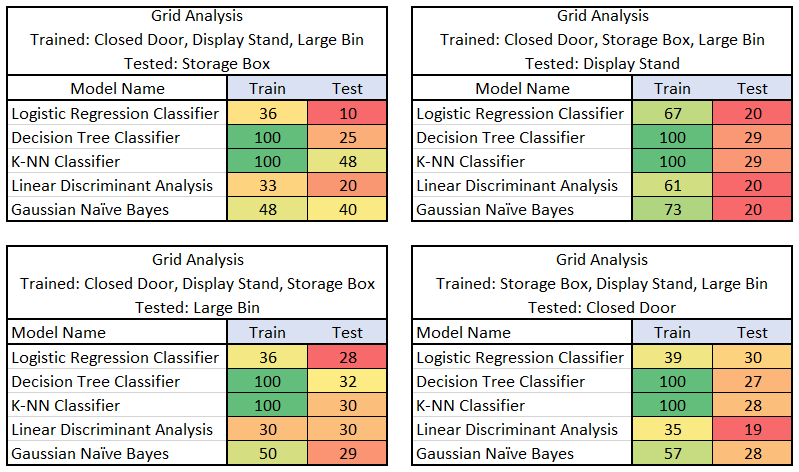
\includegraphics[width=8cm, height=7cm]{images/new_data_results.png}
\centering
\caption{Results for the Initial Binary Search}
\label{fig:new_data_results}
\end{figure}

Fig \ref{fig:new_data_results} shows that the training accuracy results for the decision tree classifier and the K-nearest neighbours algorithms are still at 100 per cent, however, there is a drop in the accuracy figures when the algorithms are presented with "new" data (i.e. data it has not been trained on).

This analysis indicates that the standard classification models, using default settings, will likely struggle to make accurate classification predictions when presented with data gathered from unseen objects. This indicates two possible paths forward. One would be to gathered data for more objects, which can be used to train the models with. This would be quite a labour-intensive task, and one can never cover all objects. Another path is to investigate the ability of neural networks to train a model. 

\subsection{Neural Networks}
Using neural networks offers a number of advantages. Neural networks can be used to learn more complex relationships, they are very well suited to classification tasks, and since they are good at learning the underlying relationships in the data, they are good with data that is not cleaned and prepared. A number of frameworks are available when working with neural networks. This work will use the Keras framework.

%Building a neural network is an iterative task: the designer will choose the metrics they wish to examine. These could include:

%\begin{itemize}
%    \item \textbf{Accuracy}: A measure of the number of correctly classified samples from the total examples in the dataset
%    \item \textbf{Precision}: A measure of the true positives (i.e. correctly identified positive samples) out of all the samples which a model has identified as positive
%    \item \textbf{Recall}: A measure of the number of true positives present in all positive samples
%    \item \textbf{F1 Score}: The F1-score sums up the predictive performance of a model using the precision and recall values
%    \item \textbf{AUC}: The Area Under the Curve is the measure of the separability, or, to put it another way, it is the measure of how well a model can distinguish between classes.
%\end{itemize}

Working with neural networks requires more work due to the need to decide on the number of layers, the number of neurons, the activation function and so on. During the neural network investigation, a number of parameters were investigated, such as using the Model and Sequential class as well as the rmsprop, Adam and SGD optimisers. The loss parameter investigated was the Sparse categorical cross-entropy, as well as the mean squared error loss. The number of epochs was varied as well at the batch size. Some investigation of the learning rate was carried out to understand the impact that can have on the accuracy. 

This investigation found that, for the grid analysis, the following parameters shown in Fig \ref{fig:nn_settings}, produced the best results

\begin{figure}[ht]
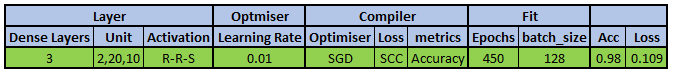
\includegraphics[width=8cm, height=1cm]{images/nn_settings.png}
\centering
\caption{Optimal Setting for Neural Network}
\label{fig:nn_settings}
\end{figure}

\subsection{System Algorithm}
One of the constraints of an embedded device, as previously mentioned, is power, another is latency. When designing a potential navigation system for people with sight difficulties, these constraints need to be kept in mind. Continually processing data at the edge will be power intensive. For this reason, it is proposed that the navigation system is split into two sections. The first would be continually processing data to determine \textit{if} an object is present. this processing would continue as long as the answer is no. When an object is detected, the system would switch to the second stage of processing, where it will determine \textit{where} the object is, thus allowing the user to navigate around it. This very simple system is shown in the flowchart in Fig. \ref{fig:embedded_algo_flowchart}:

\begin{figure}[ht]
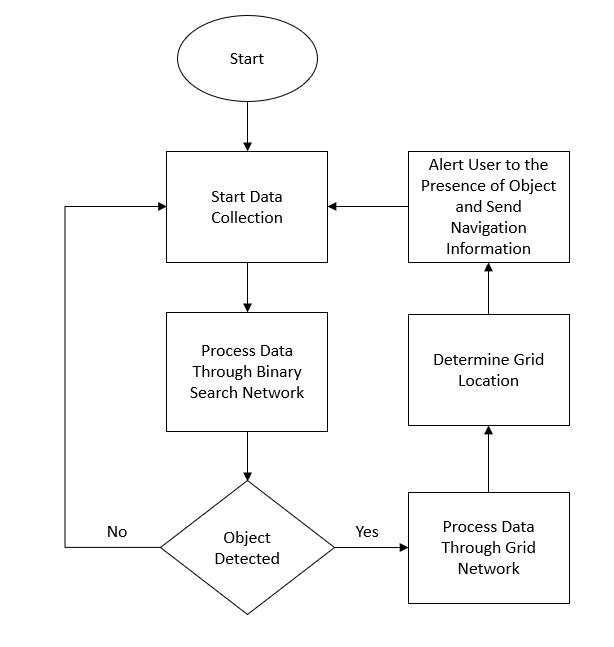
\includegraphics[width=8cm, height=8cm]{images/embedded_algo_flowchart.png}
\centering
\caption{Embedded Algorithm Flowchart}
\label{fig:embedded_algo_flowchart}
\end{figure}

The part of the flowchart which asks if an object is detected or not could be carried out by a threshold value, or potentially a series of thresholds. For example, if $x$ and $y$ are a series of decreasing values (say, 5000 and 3000), a system could be designed to ask has the first threshold been met, if the answer is yes, it then asks has the second threshold been met. If the answer is yes again, the system processes the last gathered data through the grid analysis model to detect \textit{where} the object is. 

This process could save on power as the system would not always be processing data through the grid model.

\section{Discussion}
The research set out to understand if a system could be developed which could detect obstacles in the path of a visually impaired person, in an indoor environment, allowing the user to navigate that setting. To work towards this goal, a number of tasks needed to be completed, such as the development of a data collection system and the subsequent collection of usable data from a number of obstacles. This data would then be used to train and test a number of machine learning and deep learning models to understand which is best for detecting and localising obstacles. After that, the chosen model would be implemented on a constrained device and the performance evaluated. 

Appropriate data was collected from a number of large obstacles using an Arduino development kit and two ultrasonic sensors. With the datasets in place, an initial analysis was carried out using machine learning algorithms to understand how well the data could be classified. This initial analysis indicated that these algorithms could detect both the presence of an object with a high degree of accuracy and could localise the grid location for that data. The accuracy results went down when unseen data was presented to the algorithms during the testing phase. 

This reduction in model accuracy promoted an evaluation using deep learning techniques. Various hyperparameters were evaluated during this research to understand which combination would produce the best accuracy and loss scores. 

When the neural network investigation was completed, the model was converted to a header file which was deployed on a constrained device. When tested, the model did not perform as expected. The system would carry out an inference, however, the result this inference would return did not change.

This work shows that it should be possible to implement an obstacle detection and navigation system on a constrained device due to the fact that a model was developed, which produced high accuracy scores, and deployed onto a constrained device. The issues with the incorrect inference were found in the later stages of the research and had more time been available, to allow an investigation of the issue, it is felt a solution could have been found.

\subsection{Future Work}
The inference issue on the constrained device would be the initial focus of any future research on this project. As well as this, the system algorithm which would run on the constrained device would need to be developed further to ensure it would run in as efficient a manner as possible, to allow the best use of the limited resources. 

With efficient use of resources in mind, another area for future work would further optimisation of the model which would be deployed onto the constrained device. 

There are a number of areas for further work and investigation. The first would be to understand why the deployment to the Arduino was not completely successful. 

% \section*{Acknowledgment}


% \section*{References}
\begin{thebibliography}{00}
\bibitem{b1} RNIB, "Key stats about sight loss 2021," 2021. [Online]. Available: $https://media.rnib.org.uk/documents/Key_stats_about_sight_loss_2021.pdf.$ [Accessed 3 2 2023].
\bibitem{b2} L. Pezzullo, J. Streatfeild, P. Simkiss and D. Shickle, "The economic impact of sight loss and blindness in the UK adult population," BMC Health Services Research, vol. 18, 2018. 
\bibitem{b3} Business Wire, "Global Microcontroller Market Size, Share \& Trends Analysis Report 2021-2028 - ResearchAndMarkets.com," 2021. [Online]. Available: \url{https://tinyurl.com/bdcpkuybm}. [Accessed 2 3 2023].
% \bibitem{b4} D. Situnayake and J. Plunkett, AI at the Edge, O'Reilly Media, Inc., 2023. 
% \bibitem{b5} Google, "Carol," 2021. [Online]. Available: \url{https://coral.ai/docs/som/datasheet/}. [Accessed 13 4 2023].
% \bibitem{b6} NVIDIA, "Jetson nano Development Kit," [Online]. Available: $https://developer.nvidia.com/embedded/jetson-nano-developer-kit$. [Accessed 12 4 2023].
 \bibitem{b7} NVIDIA, "Jetson nano Development Kit User Guide," [Online]. Available: \url{https://developer.nvidia.com/embedded/dlc/Jetson_Nano_Developer_Kit_User_Guide}. [Accessed 12 4 2023].
\bibitem{b8} beaglebone.org, "Beaglebone AI 64," [Online]. Available: \url{https://beagleboard.org/AI}. [Accessed 12 4 23].
\bibitem{b9} T. Sipola, J. Alatalo, T. Kokkonen and M. Rantonen, "Artificial Intelligence in the IoT Era: A Review of Edge AI Hardware and Software," 2022 31st Conference of Open Innovations Association (FRUCT), Helsinki, Finland, 2022, pp. 320-331, doi: 10.23919/FRUCT54823.2022.9770931.
\bibitem{b10} Arduino, "Arduino Nano BLE 33 Sense" [Online]. Available: \url{https://store-usa.arduino.cc/products/arduino-nano-33-ble-sense}. [Accessed 23 4 23].
% \bibitem{b11} Qualcomm, "AI is transforming everything. We are making AI ubiquitous," [Online]. Available: \url{https://www.qualcomm.com/research/artificial-intelligence}. [Accessed 12 4 23].
\bibitem{b12} TensorFlow Lite Org., "TensorFlow Lite" [Online]. Available: \url{https://www.tensorflow.org/lite/guide}. [Accessed 14 4 2023].
\bibitem{b13} TensorFlow Lite Org., "TensorFlow Lite" [Online]. Available: \url{https://www.tensorflow.org/model_optimization}. [Accessed 14 4 2023].
\bibitem{b14} TensorFlow Lite Org., "Internet of Things - Edge TPU" [Online]. Available: \url{https://cloud.google.com/edge-tpu/}. [Accessed 16 4 2023].
\bibitem{b15} K. A. B. Za’aba and L. B. Theng, "Edge Based Obstacle Detection Model Focused on Indoor Floor-Based Obstacles," 2019 IEEE 9th Symposium on Computer Applications \& Industrial Electronics (ISCAIE), Malaysia, 2019, pp. 202-207, doi: 10.1109/ISCAIE.2019.8743866.
\bibitem{b16} J. Canny, "A Computational Approach to Edge Detection," in IEEE Transactions on Pattern Analysis and Machine Intelligence, vol. PAMI-8, no. 6, pp. 679-698, Nov. 1986, doi: 10.1109/TPAMI.1986.4767851.
\bibitem{b17} R. Sattiraju, J. Kochems and H. D. Schotten, "Machine learning based obstacle detection for Automatic Train Pairing," 2017 IEEE 13th International Workshop on Factory Communication Systems (WFCS), Trondheim, Norway, 2017, pp. 1-4, doi: 10.1109/WFCS.2017.7991962.
\bibitem{b18} M. Merenda, C. Porcaro, and D. Iero, “Edge Machine Learning for AI-Enabled IoT Devices: A Review,” Sensors, vol. 20, no. 9, p. 2533, Apr. 2020, doi: 10.3390/s20092533
\bibitem{b19} S. Quinn et al., "A Thermal Imaging Solution for Early Detection of Pre-ulcerative Diabetic Hotspots," 2019 41st Annual International Conference of the IEEE Engineering in Medicine and Biology Society (EMBC), Berlin, Germany, 2019, pp. 1737-1740, doi: 10.1109/EMBC.2019.8856900.
\bibitem{b20} N. D. Lane, S. Bhattacharya, A. Mathur, P. Georgiev, C. Forlivesi and F. Kawsar, "Squeezing Deep Learning into Mobile and Embedded Devices," in IEEE Pervasive Computing, vol. 16, no. 3, pp. 82-88, 2017, doi: 10.1109/MPRV.2017.2940968.
\bibitem{b21} Amira. A. Elsonbat. (2021). Smart Blind Stick Design and Implementation. International Journal of Engineering and Advanced Technology (IJEAT), 10(5), 17–20. https://doi.org/10.35940/ijeat.D2535.0610521       
\bibitem{b22} Masaki Kuribayashi, Seita Kayukawa, Hironobu Takagi, Chieko Asakawa, and Shigeo Morishima. 2021. LineChaser: M. Kuribayashi, K. Seita, T. Hironobu, A. Chieko and M. Shigeo, "LineChaser: A Smartphone-Based Navigation System for Blind People to Stand in Lines," Proceedings of the 2021 CHI Conference on Human Factors in Computing Systems, p. 13, 2021.       
\bibitem{b23} F. Huppert, G. Hoelzl and M. Kranz, "GuideCopter - A Precise Drone-Based Haptic Guidance Interface for Blind or Visually Impaired People," Proceedings of the 2021 CHI Conference on Human Factors in Computing Systems, p. 14, 2021.      
\bibitem{b24} V. N. Mandhala, D. Bhattacharyya, B. Vamsi and N. Thirupathi Rao, "Object Detection Using Machine Learning for Visually Impaired People," International Journal of Current Research and Review, vol. 12, no. 20, pp. 157-167, 2020.      
\bibitem{b25} M. L. Mekhalfi, F. Melgani, Y. Bazi and N. Alajlan, "A Compressive Sensing Approach to Describe Indoor Scenes for Blind People," in IEEE Transactions on Circuits and Systems for Video Technology, vol. 25, no. 7, pp. 1246-1257, July 2015, doi: 10.1109/TCSVT.2014.2372371.
% \bibitem{bxx} J. Wang, S. Wang and Y. Zhang, "Artificial intelligence for visually impaired," Displays, vol. 77, p. 102391, 2023. 
\end{thebibliography}
% \printbibliography
\vspace{12pt}

\end{document}